% ============================================================
% 电路基础实验 —— 实验八 综合设计实验 预习报告
% ============================================================

\documentclass[12pt]{ctexart}

% --- 宏包 ---
\usepackage{graphicx}
\usepackage{amsmath}
\usepackage{amssymb}
\usepackage{float}
\usepackage{booktabs}
\usepackage{siunitx}
\usepackage{caption}
\usepackage{subcaption}
\usepackage{enumitem}

\sisetup{per-mode=symbol}
\DeclareSIUnit\decibel{dB}

\graphicspath{{./figures/}}

\usepackage[left=2.5cm, right=2.5cm, top=2.5cm, bottom=2.5cm]{geometry}

\setlength{\jot}{6pt}
\linespread{1.5}
\setlist{nosep}

\begin{document}

% ==================== 封面 ====================
\thispagestyle{empty}

\begin{center}
    \LARGE\textbf{第8次实验\ 综合设计实验预习报告}

    \vspace{1cm}
    \normalsize
    组名：第7组\quad 姓名：郭浩然\quad 学号：2024303980
\end{center}

\vspace{1cm}

% ==================== 正文 ====================

% (10) 实验目的
\section{实验目的}

\begin{enumerate}[label=\arabic*.]
    \item 掌握一阶有源低通滤波器与高通滤波器的电路结构和设计方法。
    \item 理解有源滤波器相对于无源滤波器在增益与阻抗匹配方面的优势。
    \item 学会将有源低通滤波器与高通滤波器级联构成带通滤波器，并确定通带频率范围。
    \item 掌握电压放大倍数与功率放大倍数的分贝定义及二者之间的换算关系。
    \item 通过 Multisim 仿真验证有源滤波器的频率特性。
\end{enumerate}

% (80) 实验原理
\section{实验原理}

\subsection{一阶有源低通滤波器}

在实验六中已学习了 RC 无源低通滤波器。无源滤波器存在通带增益始终小于 1 的固有缺陷，引入运算放大器可在实现滤波功能的同时提供信号放大能力。本实验设计的有源低通滤波器与高通滤波器电路如图~\ref{fig:design-lp-hp} 所示。

\begin{figure}[H]
    \centering
    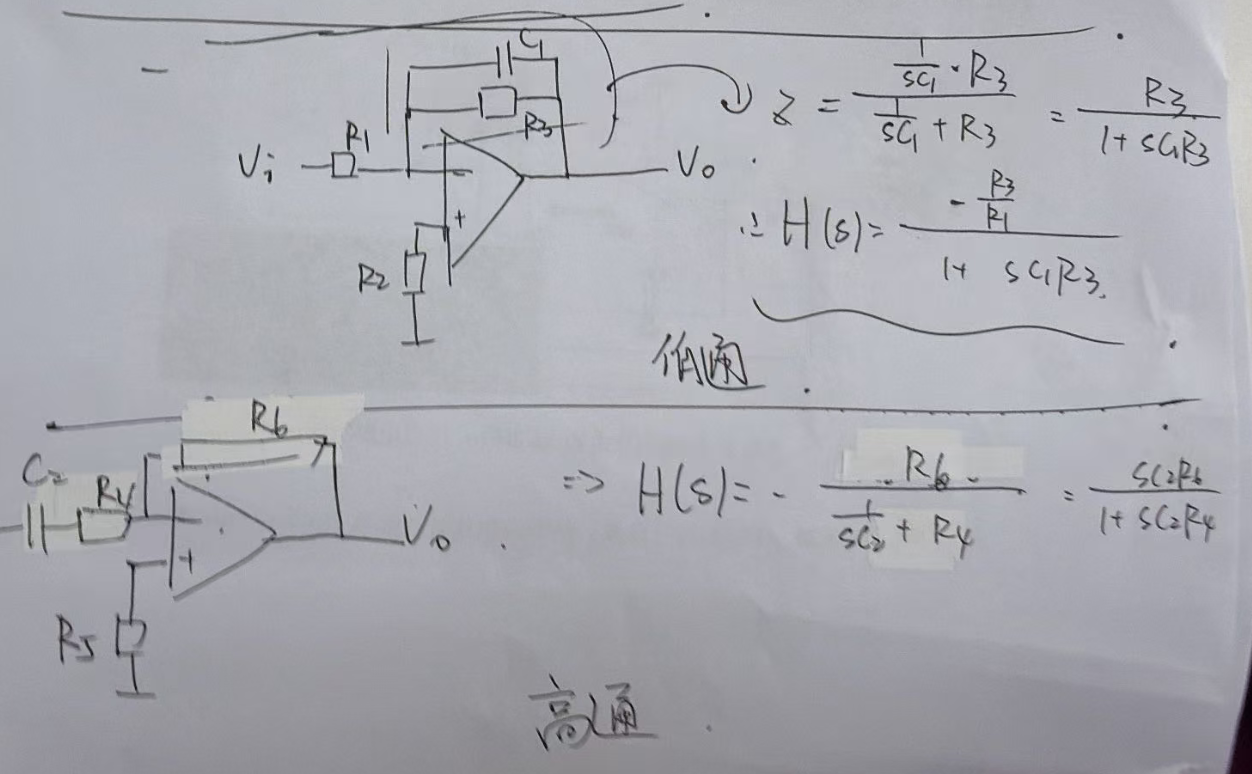
\includegraphics[width=0.7\textwidth]{手绘设计图：高通低通及传递函数.png}
    \caption{有源低通滤波器与高通滤波器电路设计}
    \label{fig:design-lp-hp}
\end{figure}

一阶有源低通滤波器如图~\ref{fig:design-lp-hp} 上部所示，基于反向比例放大器结构。将反馈支路中单一的反馈电阻替换为电阻 $R_f$ 与电容 $C$ 的并联组合，输入信号经电阻 $R_1$ 送入运放反相输入端，同相输入端接地。

利用虚短与虚断条件进行分析。输入阻抗为
\begin{equation}
    Z_1 = R_1.
\end{equation}
反馈阻抗为 $R_f$ 与 $C$ 的并联：
\begin{equation}
    Z_f = R_f \parallel \frac{1}{sC} = \frac{R_f}{1 + sR_fC}.
\end{equation}
由反向放大器增益公式 $H(s) = -Z_f / Z_1$，得传递函数
\begin{equation}
    H(s) = -\frac{R_f}{R_1} \cdot \frac{1}{1 + sR_fC}.
    \label{eq:lp-tf}
\end{equation}

令截止角频率 $\omega_{cH} = 1/(R_fC)$，对应截止频率 $f_H = 1/(2\pi R_fC)$，则幅频特性为
\begin{equation}
    |H(j\omega)| = \frac{R_f / R_1}{\sqrt{1 + \left(\dfrac{\omega}{\omega_{cH}}\right)^{\!2}}}.
    \label{eq:lp-mag}
\end{equation}

在截止频率处 $|H(j\omega_{cH})| = (R_f/R_1)/\sqrt{2}$，即通带增益下降 $3\,\mathrm{dB}$。频率远低于 $\omega_{cH}$ 时增益趋近于 $R_f/R_1$；频率远高于 $\omega_{cH}$ 时幅值以每十倍频程 $20\,\mathrm{dB}$ 的速率衰减，体现低通特性。

本实验设计中取 $R_1 = R_f = \SI{10}{\kilo\ohm}$，$C_1 = \SI{0.01}{\micro\farad}$，通带增益为
\begin{equation}
    \frac{R_f}{R_1} = \frac{\SI{10}{\kilo\ohm}}{\SI{10}{\kilo\ohm}} = 1 \quad (0\,\mathrm{dB}),
\end{equation}
截止频率为
\begin{equation}
    f_H = \frac{1}{2\pi R_f C_1}
        = \frac{1}{2\pi \times \SI{10}{\kilo\ohm} \times \SI{0.01}{\micro\farad}}
        = \frac{1}{2\pi \times 10^{-4}}
        \approx \SI{1591.5}{\hertz}.
    \label{eq:lp-fc}
\end{equation}

\subsection{一阶有源高通滤波器}

一阶有源高通滤波器如图~\ref{fig:design-lp-hp} 下部所示，同样基于反向放大器结构。将输入支路中的电阻替换为电容 $C$ 与电阻 $R$ 的串联组合，反馈支路仅包含电阻 $R_f$，同相输入端接地。

输入阻抗为电容与电阻串联：
\begin{equation}
    Z_{\mathrm{in}} = R + \frac{1}{sC} = \frac{1 + sRC}{sC}.
\end{equation}
反馈阻抗为
\begin{equation}
    Z_f = R_f.
\end{equation}
传递函数为
\begin{equation}
    H(s) = -\frac{Z_f}{Z_{\mathrm{in}}}
         = -\frac{R_f \cdot sC}{1 + sRC}
         = -\frac{R_f}{R} \cdot \frac{sRC}{1 + sRC}.
    \label{eq:hp-tf}
\end{equation}

令截止角频率 $\omega_{cL} = 1/(RC)$，则幅频特性为
\begin{equation}
    |H(j\omega)| = \frac{R_f}{R} \cdot \frac{\omega / \omega_{cL}}{\sqrt{1 + \left(\dfrac{\omega}{\omega_{cL}}\right)^{\!2}}}.
    \label{eq:hp-mag}
\end{equation}

在截止频率处 $|H(j\omega_{cL})| = (R_f/R)/\sqrt{2}$，通带增益同样下降 $3\,\mathrm{dB}$。频率远高于 $\omega_{cL}$ 时增益趋近于 $R_f/R$；频率远低于 $\omega_{cL}$ 时幅值以每十倍频程 $20\,\mathrm{dB}$ 的速率上升，体现高通特性。

本实验设计中取 $R = R_f = \SI{100}{\kilo\ohm}$，$C_2 = \SI{0.01}{\micro\farad}$，通带增益为
\begin{equation}
    \frac{R_f}{R} = \frac{\SI{100}{\kilo\ohm}}{\SI{100}{\kilo\ohm}} = 1 \quad (0\,\mathrm{dB}),
\end{equation}
截止频率为
\begin{equation}
    f_L = \frac{1}{2\pi R C_2}
        = \frac{1}{2\pi \times \SI{100}{\kilo\ohm} \times \SI{0.01}{\micro\farad}}
        = \frac{1}{2\pi \times 10^{-3}}
        \approx \SI{159.2}{\hertz}.
    \label{eq:hp-fc}
\end{equation}

\subsection{有源带通滤波器}

将有源高通滤波器与有源低通滤波器级联，可构成带通滤波器。高通级负责抑制低频成分，低通级负责抑制高频成分，二者共同限定出通带频率范围。级联电路设计如图~\ref{fig:design-bp} 所示。

\begin{figure}[H]
    \centering
    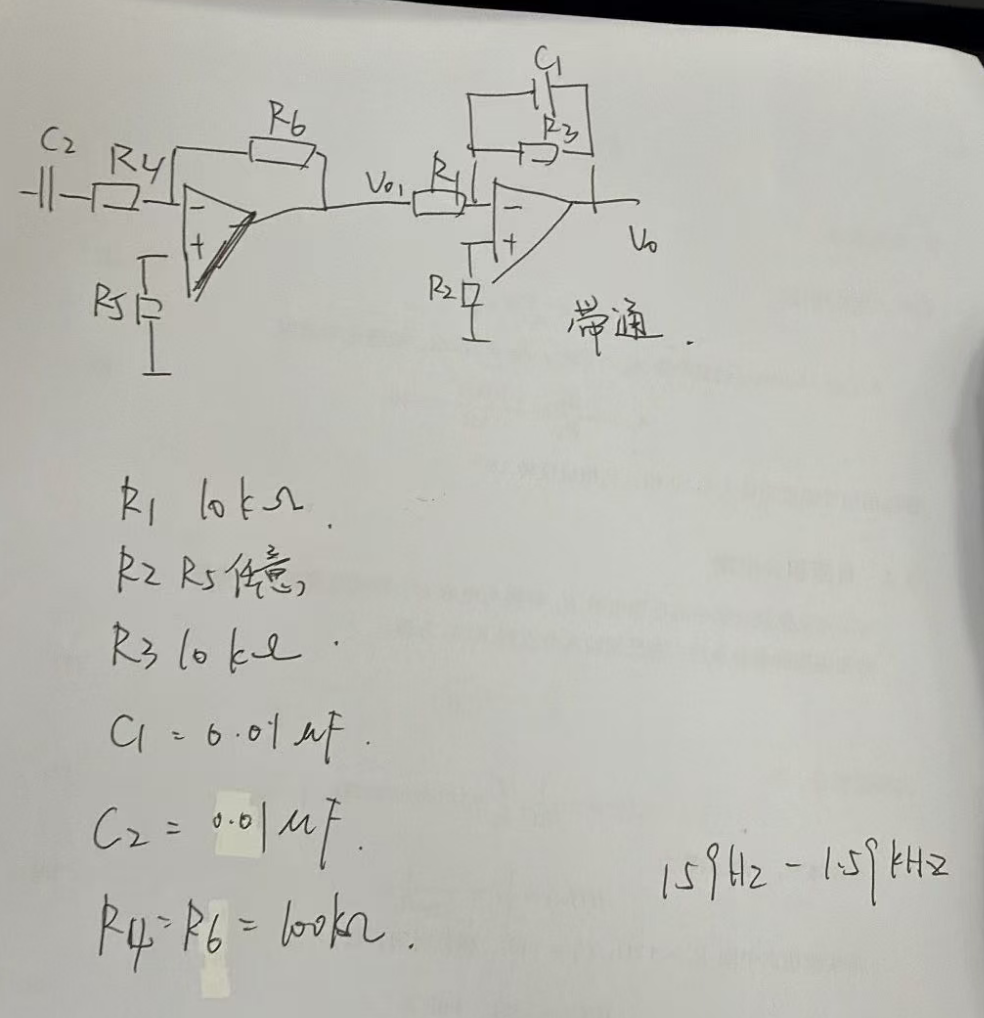
\includegraphics[width=0.7\textwidth]{手绘设计图：组合.png}
    \caption{有源带通滤波器级联设计及元件参数}
    \label{fig:design-bp}
\end{figure}

设高通级传递函数为 $H_{\mathrm{HP}}(s)$，低通级传递函数为 $H_{\mathrm{LP}}(s)$，则带通滤波器的总传递函数为
\begin{equation}
    H_{\mathrm{BP}}(s) = H_{\mathrm{HP}}(s) \cdot H_{\mathrm{LP}}(s).
\end{equation}

代入式~\eqref{eq:hp-tf} 和式~\eqref{eq:lp-tf}，并注意两级反向放大器的负号相消，得
\begin{equation}
    H_{\mathrm{BP}}(s)
    = \frac{R_{f1}}{R} \cdot \frac{R_{f2}}{R_1}
      \cdot \frac{sRC_2}{1 + sRC_2}
      \cdot \frac{1}{1 + sR_{f2}C_1}.
    \label{eq:bp-tf}
\end{equation}

两级的通带增益均为 1，故总通带增益亦为 1。通带频率范围为
\begin{equation}
    f_L \approx \SI{159.2}{\hertz} < f < f_H \approx \SI{1591.5}{\hertz}.
\end{equation}

通带宽度为
\begin{equation}
    \mathrm{BW} = f_H - f_L
               = \SI{1591.5}{\hertz} - \SI{159.2}{\hertz}
               \approx \SI{1432}{\hertz}.
\end{equation}

中心频率取几何平均值：
\begin{equation}
    f_0 = \sqrt{f_L \cdot f_H}
        = \sqrt{\SI{159.2}{\hertz} \times \SI{1591.5}{\hertz}}
        \approx \SI{503}{\hertz}.
\end{equation}

设计时需保证 $f_L < f_H$，即高通级的截止频率低于低通级的截止频率，否则两级的通带不重叠，无法构成有效的带通滤波器。

\subsection{无源滤波器与有源滤波器的比较}

\textbf{无源滤波器}仅由电阻与电容等无源元件构成。优点是电路简单，无需外部供电，工作稳定可靠，可处理大功率信号。缺点是通带内信号不可避免地被衰减，增益始终小于 1；对信号源和负载的阻抗敏感，接入负载后频率特性会发生偏移；级联时各级之间相互影响，需要专门的阻抗匹配网络；频率选择性受限于一阶 RC 网络较缓慢的衰减特性。

\textbf{有源滤波器}在无源滤波网络的基础上引入运算放大器。优点是可在滤波的同时放大信号，通带增益大于等于 1；运放的高输入阻抗与低输出阻抗使滤波器对信号源和负载的影响极小，各级可直接级联而无需额外的阻抗匹配；通过调节电阻比值可独立设定增益和截止频率。缺点是需要外部直流电源供电；运放的增益带宽积限制了滤波器的最高工作频率，通常仅适用于中低频段；有源元件会引入额外的噪声与功耗。

\begin{table}[H]
    \centering
    \caption{无源滤波器与有源滤波器的比较}
    \label{tab:filter-comparison}
    \begin{tabular}{lll}
        \toprule
        特性 & 无源滤波器 & 有源滤波器 \\
        \midrule
        通带增益   & 小于 1           & 大于等于 1，可调 \\
        电源需求   & 无需             & 需要直流电源 \\
        阻抗特性   & 受源和负载影响大 & 高输入阻抗，低输出阻抗 \\
        级联特性   & 需阻抗匹配       & 可直接级联 \\
        适用频段   & 宽，含高频       & 受运放带宽限制 \\
        电路复杂度 & 简单             & 较复杂 \\
        \bottomrule
    \end{tabular}
\end{table}

\subsection{电压与功率放大倍数的分贝表示}

分贝是一种用对数比值表示信号增益或衰减的量纲。电压放大倍数 $A_v$ 的分贝定义为
\begin{equation}
    A_{v,\mathrm{dB}} = 20\lg\frac{V_o}{V_i},
    \label{eq:av-db}
\end{equation}
其中 $V_o$ 与 $V_i$ 分别为输出电压和输入电压的幅值。同理，电流放大倍数的分贝定义为 $A_{i,\mathrm{dB}} = 20\lg(I_o / I_i)$。

功率放大倍数 $A_p$ 的分贝定义为
\begin{equation}
    A_{p,\mathrm{dB}} = 10\lg\frac{P_o}{P_i},
    \label{eq:ap-db}
\end{equation}
其中 $P_o$ 与 $P_i$ 分别为输出功率和输入功率。

两者的联系如下。设输入端阻抗为 $R_i$，输出端阻抗为 $R_o$，则
\begin{align}
    A_{p,\mathrm{dB}}
    &= 10\lg\frac{V_o^2 / R_o}{V_i^2 / R_i} \notag \\
    &= 20\lg\frac{V_o}{V_i} + 10\lg\frac{R_i}{R_o} \notag \\
    &= A_{v,\mathrm{dB}} + 10\lg\frac{R_i}{R_o}.
    \label{eq:av-ap-relation}
\end{align}

当输入端与输出端阻抗相等即 $R_i = R_o$ 时，$10\lg(R_i/R_o) = 0$，此时电压分贝数与功率分贝数在数值上相等。对于滤波器截止频率的定义，$-3\,\mathrm{dB}$ 对应电压比 $1/\sqrt{2} \approx 0.707$，功率比 $1/2 = 0.5$，即输出功率下降至输入功率的一半。

\subsection{Multisim 仿真}

根据以上设计，在 Multisim 中搭建有源带通滤波器电路。电路由高通级与低通级两个运放电路级联构成，采用 LM324AD 运算放大器，双电源供电 $V_{\mathrm{CC}} = +\SI{5}{\volt}$，$V_{\mathrm{EE}} = -\SI{5}{\volt}$。高通级使用 $C_2 = \SI{0.01}{\micro\farad}$ 与 $R = \SI{100}{\kilo\ohm}$ 确定低频截止频率；低通级使用 $R_f = \SI{10}{\kilo\ohm}$ 与 $C_1 = \SI{0.01}{\micro\farad}$ 确定高频截止频率。信号源为 $\SI{1}{V_{rms}}$ 正弦波。仿真电路如图~\ref{fig:multisim-circuit} 所示。

\begin{figure}[H]
    \centering
    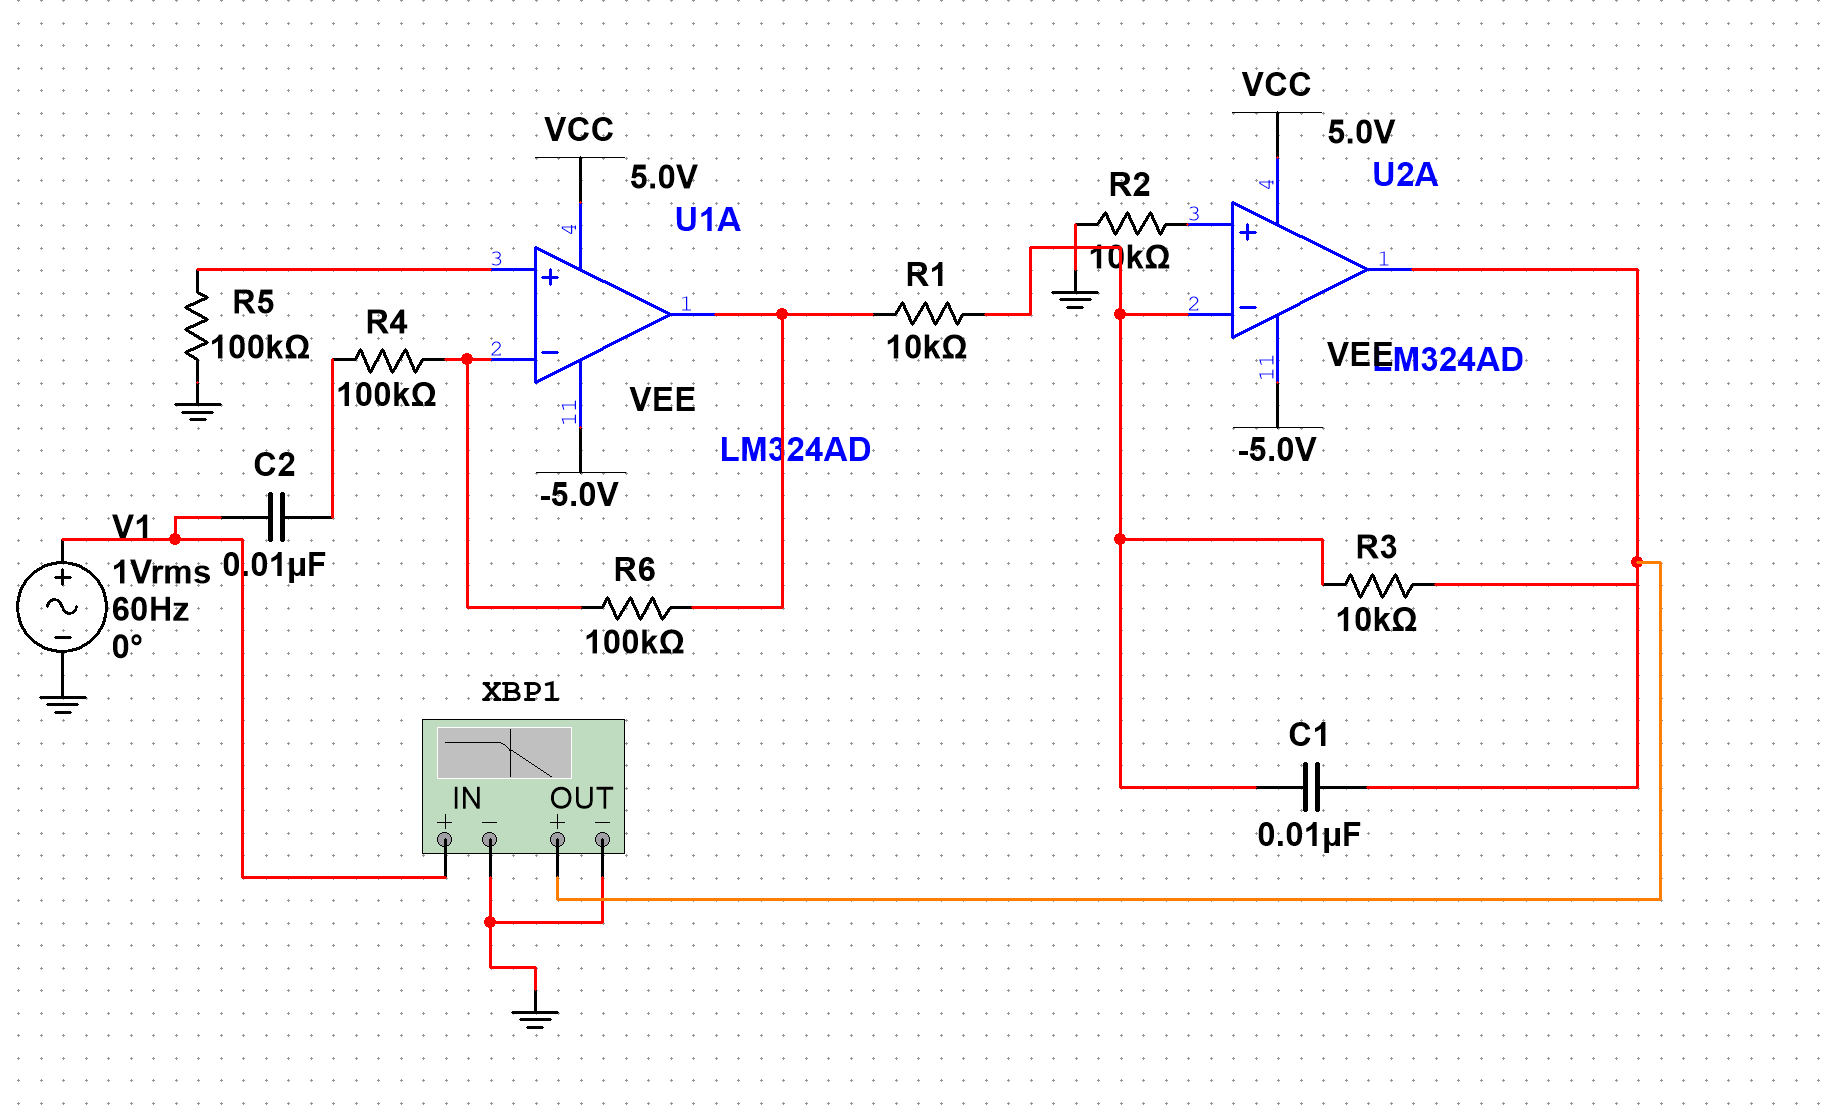
\includegraphics[width=0.85\textwidth]{multisim电路图.png}
    \caption{有源带通滤波器 Multisim 仿真电路}
    \label{fig:multisim-circuit}
\end{figure}

使用波特测试仪对电路进行扫频分析，得到带通滤波器的幅频特性曲线。图~\ref{fig:bode-plots} 分别展示了低频与高频 $-3\,\mathrm{dB}$ 截止点的测量结果。

\begin{figure}[H]
    \centering
    \begin{subfigure}[b]{0.48\textwidth}
        \centering
        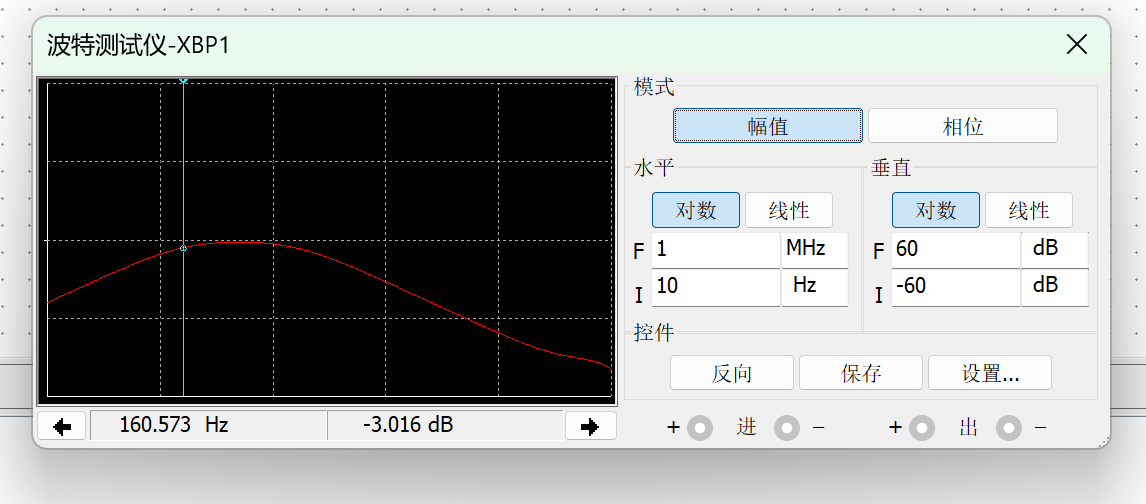
\includegraphics[width=\textwidth]{multisim波特图：低频截止.png}
        \caption{低频截止频率 $\SI{160.573}{\hertz}$，$-3.016\,\mathrm{dB}$}
        \label{fig:bode-low}
    \end{subfigure}
    \hfill
    \begin{subfigure}[b]{0.48\textwidth}
        \centering
        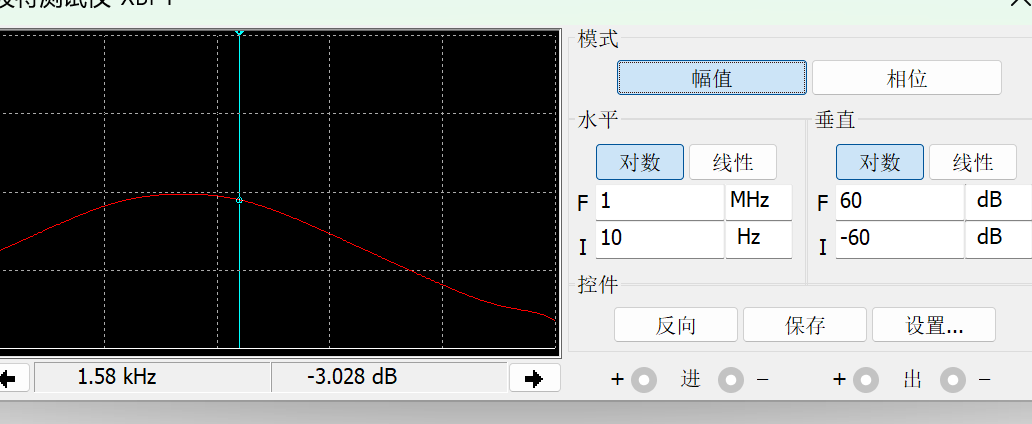
\includegraphics[width=\textwidth]{multisim波特图：高频截止.png}
        \caption{高频截止频率 $\SI{1.58}{\kilo\hertz}$，$-3.028\,\mathrm{dB}$}
        \label{fig:bode-high}
    \end{subfigure}
    \caption{带通滤波器幅频特性 $-3\,\mathrm{dB}$ 截止点}
    \label{fig:bode-plots}
\end{figure}

仿真结果与理论计算的对比如表~\ref{tab:simulation-comparison} 所示。仿真值与理论值的相对误差均小于 $1\%$，验证了电路设计的正确性。通带范围约为 $\SI{160}{\hertz}$ 至 $\SI{1.58}{\kilo\hertz}$，通带内增益接近 $0\,\mathrm{dB}$，低频段与高频段的幅值均以每十倍频程约 $20\,\mathrm{dB}$ 的速率衰减。

\begin{table}[H]
    \centering
    \caption{截止频率理论值与仿真值对比}
    \label{tab:simulation-comparison}
    \begin{tabular}{llll}
        \toprule
        截止频率 & 理论值 & 仿真值 & 相对误差 \\
        \midrule
        低频截止 $f_L$ & $\SI{159.2}{\hertz}$  & $\SI{160.6}{\hertz}$ & $0.86\%$ \\
        高频截止 $f_H$ & $\SI{1591.5}{\hertz}$ & $\SI{1580}{\hertz}$  & $0.72\%$ \\
        \bottomrule
    \end{tabular}
\end{table}

% (10) 实验器件
\section{实验器件}

\begin{itemize}
    \item 面包板 $\times 1$
    \item 直流稳压电源 $\times 1$
    \item 函数信号发生器 RIGOL DG922 $\times 1$
    \item 示波器 RIGOL DHO1204 $\times 1$
    \item 数字万用表 RIGOL DM858 $\times 1$
    \item 集成运算放大器 LM324 $\times 1$
    \item 电阻：$\SI{10}{\kilo\ohm} \times 3$，$\SI{100}{\kilo\ohm} \times 3$
    \item 电容：$\SI{0.01}{\micro\farad} \times 2$
    \item 导线若干
\end{itemize}

\end{document}
